% -*- LaTeX -*-

\documentclass[12pt,twoside]{article}
%\usepackage{healpix,psfig,html}
\usepackage{healpix,graphicx,html,makeidx}
%\usepackage{hyperref,healpix,graphicx,html,makeidx}%putting hyperref first
%screws up references in html
\begin{htmlonly}
% -*- LaTeX -*-
% This LaTeX file sets the Healpix version
% as it will appear in the documentation
% implement it with: % -*- LaTeX -*-
% This LaTeX file sets the Healpix version
% as it will appear in the documentation
% implement it with: % -*- LaTeX -*-
% This LaTeX file sets the Healpix version
% as it will appear in the documentation
% implement it with: \input{hpxversion}
% \newcommand{\hpxversion}{3.31}
% \newcommand{\hpxverstex}{3\_31}
% \newcommand{\hpxversion}{3.40}
% \newcommand{\hpxverstex}{3\_40}
% \newcommand{\hpxversion}{3.41}
% \newcommand{\hpxverstex}{3\_41}
\newcommand{\hpxversion}{3.50}
\newcommand{\hpxverstex}{3\_50}

% \newcommand{\hpxversion}{3.31}
% \newcommand{\hpxverstex}{3\_31}
% \newcommand{\hpxversion}{3.40}
% \newcommand{\hpxverstex}{3\_40}
% \newcommand{\hpxversion}{3.41}
% \newcommand{\hpxverstex}{3\_41}
\newcommand{\hpxversion}{3.50}
\newcommand{\hpxverstex}{3\_50}

% \newcommand{\hpxversion}{3.31}
% \newcommand{\hpxverstex}{3\_31}
% \newcommand{\hpxversion}{3.40}
% \newcommand{\hpxverstex}{3\_40}
% \newcommand{\hpxversion}{3.41}
% \newcommand{\hpxverstex}{3\_41}
\newcommand{\hpxversion}{3.50}
\newcommand{\hpxverstex}{3\_50}

% -*- LaTeX -*-
% This LaTeX file sets the IDL version required to run Healpix-DL
% as it will appear in the documentation
% implement it with: % -*- LaTeX -*-
% This LaTeX file sets the IDL version required to run Healpix-DL
% as it will appear in the documentation
% implement it with: % -*- LaTeX -*-
% This LaTeX file sets the IDL version required to run Healpix-DL
% as it will appear in the documentation
% implement it with: \input{idlversion}
%\newcommand{\idlversion}{5.6 }
%\newcommand{\idlversion}{6.0 }
\newcommand{\idlversion}{6.1 }

%\newcommand{\idlversion}{5.6 }
%\newcommand{\idlversion}{6.0 }
\newcommand{\idlversion}{6.1 }

%\newcommand{\idlversion}{5.6 }
%\newcommand{\idlversion}{6.0 }
\newcommand{\idlversion}{6.1 }

% -*- LaTeX -*-
% This LaTeX file sets the GDL version required to run Healpix-IDL
% as it will appear in the documentation
% implement it with: % -*- LaTeX -*-
% This LaTeX file sets the GDL version required to run Healpix-IDL
% as it will appear in the documentation
% implement it with: % -*- LaTeX -*-
% This LaTeX file sets the GDL version required to run Healpix-IDL
% as it will appear in the documentation
% implement it with: \input{gdlversion}
% \newcommand{\gdlversion}{0.9rc3 }
% \newcommand{\gdlversion}{0.9.2 }
% \newcommand{\gdlversion}{0.9.3 }
% \newcommand{\gdlversion}{0.9.6 }% Jan 2016
% \newcommand{\gdlversion}{0.9.7 }% Jan 2017
\newcommand{\gdlversion}{0.9.8}% Mar 2018
\newcommand{\gdlreldate}{March 2018}
\newcommand{\gdlsite}{https://github.com/gnudatalanguage/gdl}

% \newcommand{\gdlversion}{0.9rc3 }
% \newcommand{\gdlversion}{0.9.2 }
% \newcommand{\gdlversion}{0.9.3 }
% \newcommand{\gdlversion}{0.9.6 }% Jan 2016
% \newcommand{\gdlversion}{0.9.7 }% Jan 2017
\newcommand{\gdlversion}{0.9.8}% Mar 2018
\newcommand{\gdlreldate}{March 2018}
\newcommand{\gdlsite}{https://github.com/gnudatalanguage/gdl}

% \newcommand{\gdlversion}{0.9rc3 }
% \newcommand{\gdlversion}{0.9.2 }
% \newcommand{\gdlversion}{0.9.3 }
% \newcommand{\gdlversion}{0.9.6 }% Jan 2016
% \newcommand{\gdlversion}{0.9.7 }% Jan 2017
\newcommand{\gdlversion}{0.9.8}% Mar 2018
\newcommand{\gdlreldate}{March 2018}
\newcommand{\gdlsite}{https://github.com/gnudatalanguage/gdl}

\end{htmlonly}

% \begin{latexonly}
% \hypersetup{%
% 	pdftitle={HEALPix Installation Guidelines},%
% 	pdfauthor={E. Hivon et al},%
% 	pdfkeywords={HEALPix, Installation},%
% 	colorlinks=true}
% \end{latexonly}


\newcommand{\nside}{{N_{\rm side}}}
\newcommand{\npix}{{N_{\rm pix}}}
\newcommand{\healpixwebpage}{http://healpix.jpl.nasa.gov}
\renewcommand{\contentsname}{{TABLE OF CONTENTS}}

\newcommand{\linklatexhtml}[3]{% \linklatexhtml{name}{latex_target}{html_target}
\latexhtml{\htmladdnormallink{#1}{#2}}{\htmladdnormallink{#1}{#3}}}

%\input psfig

\sloppy
\setcounter{secnumdepth}{10}%must be non-zero for cross-reference of Figs and Sections
\setcounter{tocdepth}{10}
\newcounter{append}
%\newcounter{figure}
%\newcounter{tab}
\begin{document}

\title{\healpix Facility Installation Guidelines}
\docid{INSTALLATION GUIDE} 
\docrv{Version \hpxversion}
\author{Eric Hivon, Anthony J.~Banday, Matthias Bartelmann, Benjamin D.~Wandelt,
Frode K.~Hansen and Krzysztof M.~G\'orski}
\abstract{This document describes the installation for the \healpix facilities.}
\date{\today}

\frontpage
\tableofcontents
\newpage

\section{Introduction}

In this document the installation procedure for the \healpix
distribution is outlined. \healpix comprises a suite of Fortran 90, C++, 
IDL and Java routines
providing both stand-alone facilities and callable subroutines as an alternative
for those users who wish to build their own tools.
A set of C subroutines and functions is also provided. 

The distribution can be downloaded as a gzipped and tarred file,
which can be unpacked by executing the commands \hfill\newline
%\begin{verbatim}
{\tt \% gunzip Healpix\_\hpxversion.tar.gz}\hfill\\
{\tt \% tar -xpf Healpix\_\hpxversion.tar}\hfill\\
%\end{verbatim}

\begin{figure}[!ht]
%\centerline{\psfig{figure=fig/dir_tree.eps,width=\textwidth}}
\latexhtml{%for latex
\centerline{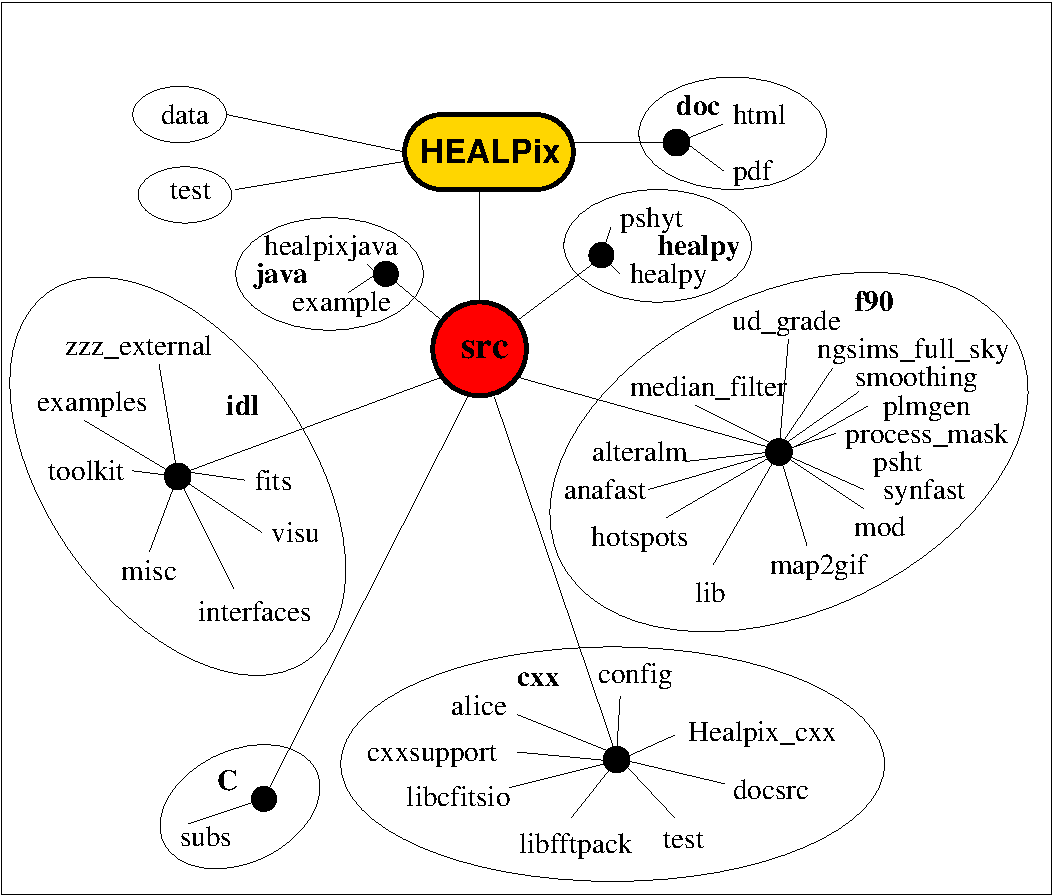
\includegraphics[bb=0pt 0pt 562pt 478pt,width=\textwidth,clip]{fig/dir_tree.pdf}}
}{%for html
%\centerline{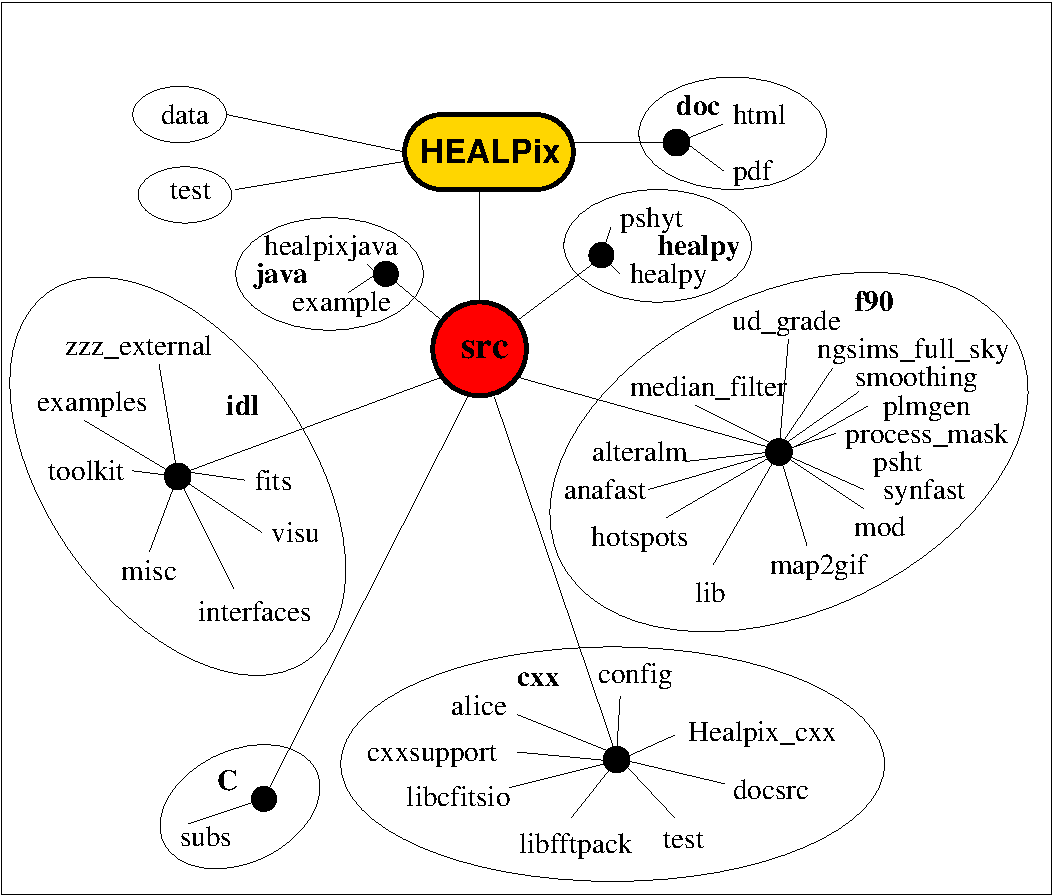
\includegraphics[bb=1pt 1pt 562pt 478pt,width=\textwidth]{fig/dir_tree.eps}\htmlimage{}}
\centerline{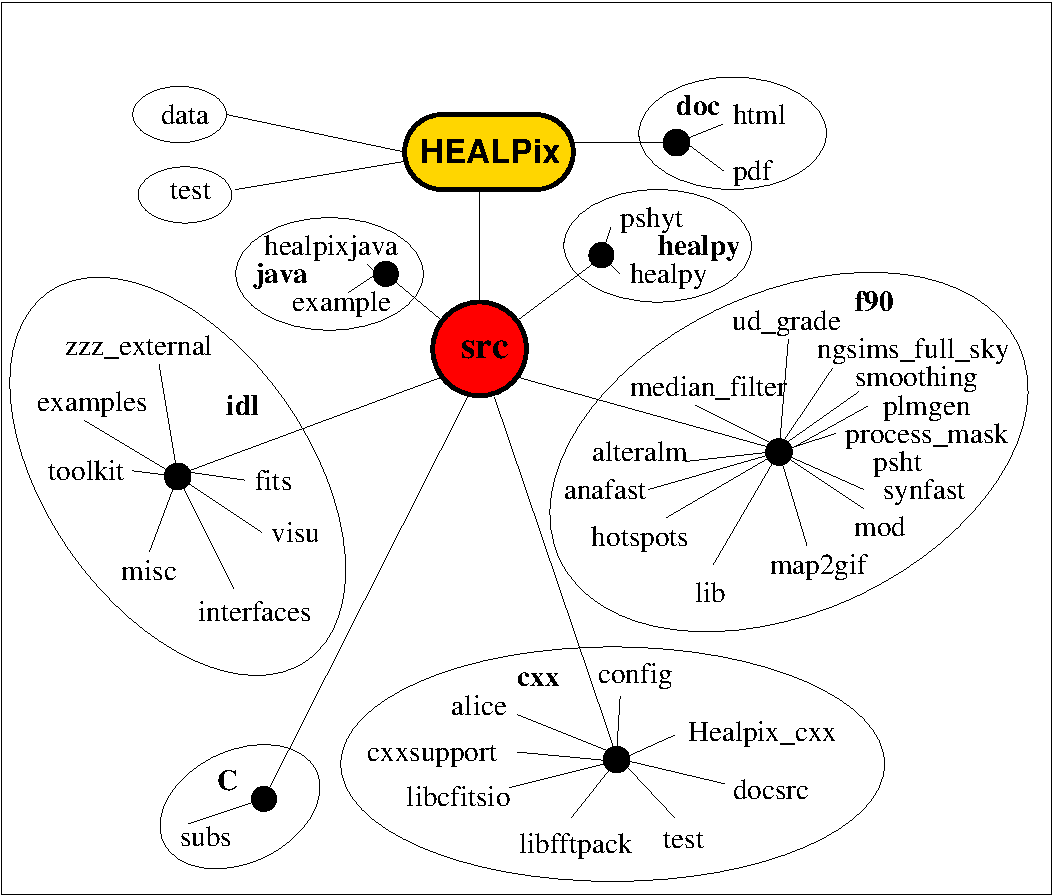
\includegraphics[width=0.5\textwidth]{fig/dir_tree}}
}

\caption[Directory structure]{%
\label{page:dirtree}
\label{fig:dirtree} % put \label *IN* \caption !!!!!
The directory structure for the \healpix distribution. }
\end{figure}

The unpacked distribution has a directory structure as shown in Figure
\ref{fig:dirtree}.

As with most freely available software, the distribution
comes with caveats, the major one being that although we have attempted
to automate the installation as much as possible, not all eventualities
can ever be foreseen. We have tested the installation on the following 
platforms: \hfill\newline
\noindent AIX, IRIX, IRIX64, Linux, SunOS, ALPHA and Darwin (MacOS) \hfill\newline

There may be problems in the facility build due to the local system 
configuration which is beyond our control. 

\section{Installation Requirements}
\label{sec:requirements}
The major part of the \healpix distribution is written in both \textbf{Fortran 90} and \textbf{C++} and
so the appropriate compiler(s) must be present (Linux and Darwin users should look
at Section~\ref{sec:freef90compilers} about free F90 compilers. Microsoft Windows
users should look at Section~\ref{sec:windows}). Many visualisation tools and map
manipulation routines are provided in \textbf{IDL} (please note 
that at least version \idlversion is required) and \textbf{Java}. Some of the \healpix routines are
also available in \textbf{C}.

{\em This section and the next focus on the compilation and installation of the
  \textbf{C}, \textbf{C++}, \textbf{Fortran~90}  and \textbf{IDL} routines. For more information on the 
\textbf{Java} routines see table~\ref{tab:allpackages}}

\begin{table}[!h]
\begin{tabular}{p{0.15\hsize} p{0.35\hsize} p{0.4\hsize}} \hline  
  \textbf{Healpix Package} & \textbf{Information on installation} &
\textbf{Information on routines}\\ \hline
                            &                      &     \\ %%% for presentation
%
  Fortran 90     & This document & 
\linklatexhtml{''Fortran Facilities''}{facilities.pdf}{facilities.htm} and 
\linklatexhtml{''Fortran Subroutines''}{subroutines.pdf}{subroutines.htm} documents \\
%
 & & \\
%
  IDL            & This document  & 
\linklatexhtml{''IDL Facilities''}{idl.pdf}{idl.htm}\\
 & & \\
%
  C++     & This document, or \phantom{filling up --} {\tt src/cxx/README.compilation} & 
%\htmladdnormallink{''C++ Facilities and Subroutines''}{index_cxx.html}
\linklatexhtml{''C++ Facilities and Subroutines''}{../html/index_cxx.html}{index_cxx.html}
 (HTML only)\\
%
 & & \\
%
  java    & {\tt src/java/README} & 
%\htmladdnormallink{''Java Overview''}{java/index.html}
\linklatexhtml{''Java Overview''}{../html/java/index.html}{java/index.html}
 (HTML only)\\
%
 & & \\
%
  C       & This document, or \phantom{filling up --} {\tt src/C/README} & 
    \linklatexhtml{''C Subroutines Overview''}{csub.pdf}{csub.htm} \\ 
%
                                   &                          \\ \hline %%% for presentation
\end{tabular}
\caption[Documentation]{%
\label{tab:allpackages}  % put \label *IN* \caption !!!!!
Documentation on the installation and usage of the different packages}
\end{table}

The configure script is written in the Bourne shell. The script
attempts to generate a {\tt Makefile} which is tailored to one of 
the above Operating Systems (OS's) and using 
{\tt Makefile.in} as a template for non system-specific statements. 
Only the basic UNIX make facility is required to build the software, although we do
still recommend the GNU make facility (\htmladdnormallink{{\tt ftp://ftp.gnu.org/gnu/make/}}{ftp://ftp.gnu.org/gnu/make/}).
In addition, several environment configuration files and an IDL startup file are
generated. These automatically establish
various environment variables and aliases to make the use of the
\healpix package simpler. 

The \healpix \textbf{Fortran 90}, \textbf{C++} and \textbf{C} distributions also require the publicly available CFTISIO
library:

\begin{tabular}{p{0.3\hsize} p{0.6\hsize}} \hline  
  \textbf{Software Package} & \textbf{Source} \\ \hline
                            &                          \\ %%% for presentation
  CFITSIO V 2.xx or 3.xx library            & \htmladdnormallink{{\tt
                            http://heasarc.gsfc.nasa.gov/docs/software/fitsio/}}
			{http://heasarc.gsfc.nasa.gov/docs/software/fitsio/}
                            \\ 
                                   &                          \\ \hline %%% for presentation
\end{tabular}\vspace{3ex}

The \textbf{IDL} visualization software is commercially
available at

\begin{tabular}{p{0.3\hsize} p{0.6\hsize}} \hline  
  \textbf{Software Package} & \textbf{Source} \\ \hline
                            &                          \\ %%% for presentation
IDL V \idlversion or more          & \htmladdnormallink{{\tt
                            http://www.ittvis.com/}}{http://www.ittvis.com/}
			\\
                                   &                          \\ \hline %%% for presentation
\end{tabular}\vspace{3ex}

while the GNU Data Language \textbf{GDL}, a {\em free} clone of IDL 6.0, can also be used (with some
caveats, see \S\ref{sec:using_gdl}) and can be downloaded for free from

\begin{tabular}{p{0.3\hsize} p{0.6\hsize}} \hline  
  \textbf{Software Package} & \textbf{Source} \\ \hline
                            &                          \\ %%% for presentation
GDL \gdlversion or more         & \htmladdnormallink{{\tt
                            http://sourceforge.net/projects/gnudatalanguage/}}{%
			http://sourceforge.net/projects/gnudatalanguage/}
			\\
                                   &                          \\ \hline %%% for presentation
\end{tabular}\vspace{3ex}



%\vspace{3ex}

%(versions 5.3 to 6.2 have been extensively used during the development
%of the \healpix IDL codes).
As it was already the case in version 1.20, users no longer need to acquire the IDL
Astronomy User's Library (\htmladdnormallink{{\tt http://idlastro.gsfc.nasa.gov/homepage.html}}{http://idlastro.gsfc.nasa.gov/homepage.html})
or the COBE (IDL) Analysis Software (\htmladdnormallink{{\tt http://lambda.gsfc.nasa.gov/product/cobe/cgis.cfm}}{http://lambda.gsfc.nasa.gov/product/cobe/cgis.cfm}),
although we do recommend these packages to the user.
The 100-odd routines required for version \hpxversion\ are contained in the
subdirectory {\tt Healpix\_\hpxversion/src/idl/zzz\_external}.
These procedures are included in the \healpix package unchanged and 
solely for the purpose of making it self contained. In this way,
we remove the burden of installation of additional libraries from 
the end user.

% For convenience we provide the freely available FFTPACK\footnote{At 
% {\tt
% http://math.nist.gov/cgi-bin/gams-serve/list-package-components/FFTPACK.html}}
% routines ''rffti'', ''rfftf'' and ''rfftb''.
%

%% At the user choice (at installation time) the FFT operations can be
%% performed with the FFT code shipped with the package, or with the
%% freely available FFTW. In the latter case FFTW should be compiled in
%% double precision.

A parallel implementation (based on OpenMP, for shared memory architectures) of the Spherical Harmonics
Transforms involved in {\tt synfast, anafast, smoothing, plmgen} and {\tt alteralm} is now
available by default and can be readily compiled and used with the standard installation script. 

A set of routines with MPI parallelization (for distributed memory architectures)
 is also available for Spherical Harmonics Transform, thanks to the work of H.K. Eriksen
 (h.k.k.eriksen@astro.uio.no) and Snorre Boasson (ITEA, NTNU). See the F90
 subroutines documentation for more information on how to use those routines in
 your code.
%% , thanks to the work of St\'ephane Colombi. It has
%% only been tested on SGI and DEC computers.
%% At this point, it can \textbf{not} be used together with FFTW.

We found that it was remarkably difficult to find 
random number generators in the public
domain which are simple yet
powerful and easy to use. 
We are providing one (both in C++ and F90) which is an adaptation of an xorshift generator described
 in Marsaglia (Journal of Statistical Software 2003, vol 8). It has a theoretical period of $2^{128}-1 \approx 3.4\ 10^{38}$.

%% One of us (BDW) has therefore attempted to create one and we
%% provide it as free software with this package (cf. Appendix I).

\section{The Installation Procedure}

If the user has one of the supported OS's, then installation proceeds utilizing
the following commands. If your OS is not supported, the configuration step
should be omitted, {\tt Makefile.in} should be copied as {\tt Makefile} and explicitly
tailored to the user environment.


\begin{flushright}
\begin{tabular}{p{0.3\hsize} p{0.60\hsize}}
{\tt \% ./configure} {\em [-L]}    & uses {\tt Makefile.in} as a template to build 
                         the correct Makefile (from user inputs as required), it
                         will also configure the IDL routines\\
{\tt \% make}           & builds all the facilities \\
{\tt \% make test}      & tests all the facility previously compiled \\
{\tt \% make clean}     & removes object files \\
%%%%%{\tt \% make vclean}    & 
{\tt \% make tidy}      & removes object files, executables and libraries \\
{\tt \% make distclean} & same as above and restores the directories to the state of the 
                          original distribution \\
%% {\tt \% ./config\_preview} & configure the IDL previewer
\end{tabular}
\end{flushright}
These different steps are detailled below.

\subsection{./configure [-L]}

The {\tt ./configure} script manages the configuration of the C, C++,
Fortran90 and IDL suites of routines and facilities.

Since v2.11, it accepts the {\tt -L} option to write the \healpix specific configuration files
into the \healpix directory itself rather than in installer's home directory (see
\S~\ref{subsub:conf}).
Using the {\tt -L} option is recommended when doing a {\em project} or {\em system wide} installation of
\healpix to be accessed by several different users.

An online help is available with {\tt ./configure -h}.

\subsubsection{Configuration profile}
\label{subsub:conf}
A feature introduced in previous releases and enhanced since v2.10, is that 
the configure script creates a shell configuration file \hfill\\
(located in
{\tt \$\{HOME\}/.healpix/2\_12\_}{\em $\langle$OS\_TYPE$\rangle$}{\tt /config}
or in
\hfill\\
{\tt \$\{HEALPIX\}/confdir/2\_12\_}{\em $\langle$OS\_TYPE$\rangle$}{\tt /config}
if {\tt ./configure -L} was used)
according to shell
type in which various environment variables and aliases are defined
for your convenience. If you agree upon prompting, it will also
change your default system profile during installation to
automatically source this profile. If you do not agree to this change,
you will need to explicitly source the configuration file above for any session in
which you intend to run \healpix facilities. {\bf In particular, you will
have to make sure that the {\tt HEALPIX} system variable is correctly
defined (as the full path to the \healpix directory) before running
the package}.

% And finally, the current {\tt ./configure} script allows several compilations of
% the Healpix routines to coexist by letting the user choose the name of directories
% containing the executables, libraries and include files.

\subsubsection{C configuration}

The {\tt ./configure} script will ask for the C compiler and options to
be used, and for the full path of an installed {\tt cfitsio} library to link to.
By default, only a static library is created, but the user can also ask for
 a shared (Unix/Linux systems) or dynamic (Darwin) library. \\
After compilation
(see {\tt make} section) and linking, all libraries will be 
in {\tt \$\{HEALPIX\}/lib/chealpix.*}\ .

\subsubsection{C++ configuration}

The {\tt ./configure} script will 
ask for the full path to an installed {\tt cfitsio} library to link to, and then provide a choice of
predefined targets corresponding to different combinations of C++ compilers and
options. Each of those targets is defined in a configuration file located in
{\tt Healpix\_\hpxversion/src/cxx/config/config.}{\em target}.
The user can therefore add new targets or edit existing ones, and the
{\tt ./configure} script will update its menu accordingly.
If a fairly recent version
(4.2 or higher) of gcc and g++ is installed on the system, the target
"generic\_gcc" should always work, except under MacOSX, where ``osx'' target is
required.  \\
The environment variables EXTERNAL\_CFITSIO, 
CFITSIO\_EXT\_LIB, 
CFITSIO\_EXT\_INC and 
HEALPIX\_TARGET 
will be set according to the choices made above.
\\
If the HEALPIX configuration file is sourced as described in \S~\ref{subsub:conf}, the full path to the C++
executables will be added to the environment PATH variable.


\subsubsection{Fortran 90 configuration}
When you run {\tt ./configure} on a supported system 
you will be prompted to enter compiler optimisation flags.
We have not attempted to provide the best optimisation flags for all
operating systems. The configure
script will have a guess at optimisation options for some systems, but it
is up to the user to figure out an optimal set\footnote{In particular, the Intel Fortran
Compiler, available for free for PC's with Intel-like processors, have a set of
optimization options for each of Intel processor families (Pro, II, MMX, 4). Please consult
the online help ({\tt ifort -help}) or PDF documentation ({\tt
/opt/intel\_fc\_80/doc/} or {\tt /opt/intel/fc/9.*/doc}) or HTML documentation
({\tt /opt/intel/fce/10.*/doc/Doc\_Index.htm}) for further information.}. From our experience,
we have not found significant accumulation of numerical error even
when using the most aggressive optimisation level available. \\
If the HEALPIX configuration file is sourced as described in \S~\ref{subsub:conf}, the full path to the F90
executables will be added to the environment PATH variable.

\subsubsection{IDL configuration}
You will be asked for the external applications you want to use to visualize the
Postscript and PNG files created by IDL. \\
If the HEALPix configuration file is
sourced as described in \S~\ref{subsub:conf}, the aliases {\tt hidl} and {\tt hidle}
are also defined to give you access to HEALPIX routines from IDL.


\subsection{Compilation and installation}

The \\
\mycode{make} \\
command will compile one or several of the C, C++ and F90 packages
depending on what was configured with the {\tt ./configure} script.
Specific packages can be compiled with the respective commands 
\begin{verbatim}
   make c-all
   make cpp-all
   make f90-all.
\end{verbatim}

To perform several compilation jobs simultaneously, the command {\tt make -j [jobs]}
can be used.

Please neglect any possible warnings at compile time. If you run into
trouble please refer to the section \htmlref{{\bf Troubleshooting and further
information}}{sec:troubleshoot}.

After running {\tt make}, the user must re-login to ensure that the new profiles built by the installation
procedure are correctly sourced. Only then will the
user have full access to the specific \healpix
environment variables etc.

\subsection{Testing the installation}

All installed libraries and executables can be tested with 
\begin{verbatim}
   make test
\end{verbatim}

while specific tests of the C, C++ and Fortran products can be performed with,
respectively
\begin{verbatim}
   make c-test
   make cpp-test
   make f90-test
\end{verbatim}
For the latter, Table~\ref{tab:f90_tests} lists the codes tested with the
parameter files used, as well as the data files produced and the respective
reference files.

\begin{table}[!h]
\begin{tabular}{l l l l l}
\hline
{\bf code}    \& parameter file & output data 		& reference data & output image & reference image \\
\hline
{\bf synfast}  syn.par & test\_map.fits 	& map.fits 	& test\_map.gif & map.gif \\
              & test\_alm.fits 	& alm.fits 	& {\em NA} & {\em NA} \\
{\bf smoothing}  smo.par & test\_sm.fits	& map\_sm.fits	& test\_sm.gif & map\_sm.gif \\
{\bf ud\_grade}  udg.par & test\_LOres.fits	& map\_LOres.fits & test\_LOres.gif	& map\_LOres.gif \\
{\bf hotspot}  hot.par & test\_ext.fits	& map\_ext.fits & test\_ext.gif	& map\_ext.gif \\
		       & test\_max.asc	& max.asc & {\em NA} & {\em NA} \\
		       & test\_min.asc	& min.asc & {\em NA} & {\em NA} \\
{\bf anafast}  ana.par & test\_cl.fits	& cl\_out.fits & {\em NA}	& {\em NA} \\
{\bf alteralm}  alt.par & test\_almdec.fits	& almdec.fits & {\em NA}	& {\em NA} \\
{\bf median\_filter}  med.par & test\_mf.fits	& map\_mf.fits	& test\_mf.gif & map\_mf.gif \\
{\bf sky\_ng\_sim}  ngfs.par & test\_ngfs.fits	& map\_ngfs.fits	& test\_ngfs.gif & map\_ngfs.gif \\
\hline
\end{tabular}
\caption[Data files]{
\label{tab:f90_tests} % put \label *IN* \caption !!!!!
Data files and images produced by the Fortran codes during the tests,
and the respective reference files to which they can be compared. All the files listed
are located or produced in the {\tt Healpix\_\hpxversion/test} directory. The GIF images of full sky maps were
produced using {\tt map2gif}. {\em NA}: No image available, because the data set is not a sky map}
\end{table}


{\bf{Notes:}} 
\begin{itemize}
\item the input power spectrum (in {\tt
Healpix\_\hpxversion/test/cl.fits}) used to generate the Fortran90 test maps
is currently the WMAP 1yr best fit, in $(\mu$K$)^2$, and is therefore different from the one
included in releases 1.* (that can still be found in {\tt cl\_old.fits}).
See \htmladdnormallink{{\tt  http://lambda.gsfc.nasa.gov/}}{http://lambda.gsfc.nasa.gov/} 
for details on WMAP and its data products.
%
\item the file  {\tt Healpix\_\hpxversion/test/wmap\_lcdm\_sz\_lens\_wmap5\_cl\_v3.fits}
 was added for convenience, even though
 it is currently *NOT* used for any of the simulated test maps.

 It has been adapted to run with \healpix  from WMAP 5yr best fit model for
$\Lambda$-CDM + SZ + lensing with B mode = 0, in $(\mu$K$)^2$ (input file: 
\htmladdnormallink{{\footnotesize{\tt  http://lambda.gsfc.nasa.gov/data/map/dr3/dcp/params/c\_l/wmap\_lcdm\_sz\_lens\_wmap5\_\-cl\_v3.dat}}}{http://lambda.gsfc.nasa.gov/data/map/dr3/dcp/params/c_l/wmap_lcdm_sz_lens_wmap5_cl_v3.dat}).
 For the value of the cosmological parameters, see 
 \htmladdnormallink{{\footnotesize{\tt  http://lambda.gsfc.nasa.gov/product/map/dr3/params/lcdm\_sz\_lens\_wmap5.cfm}}}{%
http://lambda.gsfc.nasa.gov/product/map/dr3/params/lcdm_sz_lens_wmap5.cfm}
\end{itemize}

In order to test the new \healpix profile set-up one can then attempt
to run any C++ or F90 facility from any directory on your system. Similarly,
IDL should be tested by invoking {\tt hidl} or {\tt hidlde}.



\subsection{Cleaning up}
Three levels of cleaning are available:
\begin{verbatim}
  make clean
\end{verbatim}
will remove the intermediate files created during compilation, such as object
files, (Fortran) modules files, ... found in the source or build directories;
\begin{verbatim}
  make tidy
\end{verbatim}
same as above, and will also remove the \healpix executables, libraries and module and/or
include files;
\begin{verbatim}
  make distclean
\end{verbatim}
will return the \healpix directory to its original 'distribution' state by discarding the same
files as above, as well as the executable and library directories and the top
level Makefile.

\section{Upgrading from 2.0 to 2.1}

The internal structure of release 2.1 is quite different from release 2.0 and to
avoid confusion during the compilation we highly recommend to put the new
release in a {\em different} directory, rather than putting the new package on
top of the old one. 
If you actually change the name of the 'active' \healpix directory care must be taken that
all references to the old directory are removed from your system profile before
adding the new ones (see Note on {\it Re}-installation).

% \section{Upgrading from 2.10 to 2.11}

%% See the \htmladdnormallink{\healpix Primer}{intro.htm} for a note on the change of convention for polarization.

\section{A Note on {\it Re}-installation}

As a result of the line added to your shell profile which explicitly
sources the \healpix profile, care must be taken if the package 
is reinstalled in a different directory. If such reinstallation
is desired, the included line must be removed from your system profile,
allowing the corrected version to be added.  

\section{Troubleshooting and further information}
\label{sec:troubleshoot}
This section contains a list of difficulties which we have dealt
with. It is by no means exhaustive. A troubleshooting forum has
been established at \htmladdnormallink{{\tt \healpixwebpage/healpixSoftwareProblemsBugsSolutions.shtml}}{\healpixwebpage/healpixSoftwareProblemsBugsSolutions.shtml}, where we 
list current questions and solutions to known problems (for
a given release). A bug tracker is also available on SourceForge \htmladdnormallink{at this address}{http://sourceforge.net/tracker/?group_id=130539&atid=718128}.
If the problem you encounter is not addressed in those forums nor below, 
please contact 
{\em healpix} {\tt at} {\em jpl.nasa.gov}


\subsection{Installation under Microsoft Windows}
\label{sec:windows}
The installation and usage of HEALPix require many standard Unix/Linux tools
(such as {\tt sh, make, awk, grep, sed, ls, wc, cat, more, nm, ar}) as well as C,
C++ and Fortran compilers. To install it under Windows, you will need to
\begin{itemize}
\item Install Cygwin on your machine 
(see \htmladdnormallink{{\tt http://cygwin.com/}}{http://cygwin.com/}).
In addition to the default packages, you need at least the {\tt binutils,
    coreutils, util-linux, bash, gawk, grep, make} and {\tt sed} packages, as
    well as {\tt gcc} and {gcc-g++} packages, all available at 
\htmladdnormallink{{\tt http://cygwin.com/packages/}}{http://cygwin.com/packages/}.
\item Install the latest gfortran binaries for Cygwin from 
\htmladdnormallink{{\tt http://quatramaran.ens.fr/$\tilde{}$coudert/gfortran/}}{%
http://quatramaran.ens.fr/~coudert/gfortran/}, 
following the instructions at 
\htmladdnormallink{{\tt http://gcc.gnu.org/wiki/GFortranBinaries}}{%
http://gcc.gnu.org/wiki/GFortranBinaries}.
\item Unpack the HEALPix software package
\item Run configure as you would on other platforms
\item The C++ code can be compiled using HEALPIX\_TARGET=generic\_gcc
\end{itemize}

\subsection{Problems with CFITSIO}
\subsubsection{Compilation of CFITSIO Fortran wrappers}
The most common problem with the Fortran \healpix compilation will produce
messages like:
\begin{verbatim}
  ld: Undefined symbols:
   _ftbnfm_
   _ftclos_
   _ftcrhd_
   _ftdkey_
   ...
\end{verbatim}
or
\begin{verbatim}
  fitstools.f90: undefined reference to `ftdkey_'
  fitstools.f90: undefined reference to `ftbnfm_'
  fitstools.f90: undefined reference to `ftclos_'
  ...
\end{verbatim}
or
\begin{verbatim}
 Undefined symbols:
  "_ftghbn_", referenced from:
      ___fitstools_MOD_read_fits_cut4.clone.2 in libhealpix.a(fitstools.o)
      ___fitstools_MOD_getsize_fits.clone.1 in libhealpix.a(fitstools.o)
      ___fitstools_MOD_getsize_fits in libhealpix.a(fitstools.o)
   ...
 ld: symbol(s) not found
 collect2: ld returned 1 exit status
\end{verbatim}
and occurs when the CFITSIO installation script could not find a valid fortran compiler.\\
To solve this problem
\begin{enumerate}
\item Go into the CFITSIO directory. \\
Assuming that {\bf ifort} is available on your
system (it can be replaced below by {\tt \bf gfortran}, {\tt \bf g95}, {\tt \bf f77}, {\tt \bf f2c}, $\ldots$) type: \\
\mycode{./configure FC={\bf ifort}} \\
\mycode{make} \\
\mycode{make install} \hskip 0.3cm (optional).
%
\item Then go back into the \healpix directory and do \\
\mycode{./configure} \hskip 0.3cm (making sure that you are using the newly created {\tt libcfitsio.a} library) \\
\mycode{make} \\
\mycode{make test}
\end{enumerate}
See also the note below on 64 bit architectures.

\subsubsection{CFITSIO problems on systems with 64 bit architecture}

\begin{enumerate}
%
\item {\bf Linux, Mac OS X}

If the \healpix codes are compiled in 64 bits, and the GNU C Compiler ({\tt
gcc}) is used to compiled CFITSIO, then issue the following commands in the
CFITSIO directory:

\begin{verbatim}
  ./configure FC='gcc -m64'
  make
\end{verbatim}

You can
then force compilation to the same binary format by entering
{\tt -m64} when asked for the optimisation options in the
\healpix configure script.

\item {\bf IRIX64}

On a 64-bit architecture such as IRIX64, CFITSIO will have to be
compiled in the same  binary format as the \healpix codes.
This can be achieved by typing the
following on the
command line in the CFITSIO directory:
 
\begin{verbatim}
  rm config.cache    
  setenv CC 'cc -n32'
  ./configure
  make
\end{verbatim}

Alternatively you can replace the {\tt -n32} with {\tt -64}. You can
then force compilation to the same binary format by entering either
{\tt -n32} or {\tt -64} when asked for the optimisation options in the
\healpix configure script.
%
\end{enumerate}

\subsubsection{CFITSIO linking problems}

A particular problem encountered with the CFITSIO Version 2.0 release relates
to the inclusion of various libraries within the system release for a given
machine. This led to some modifications to the Makefile to include the specific
library links {\tt -lm -lnsl -lsocket} on SunOS, but only {\tt -lm} for IRIX64.
If your OS is not completely supported by the distribution, you may find this
as one source of errors. The CFITSIO developers recommend compilation of the
{\tt testprog} routine. Inspection of the libraries linked after executing the
{\tt make testprog} statement will reveal those you need to include in the
Makefile.

\subsubsection{CFTISIO and Debian/Linux}

Some problems have been reported on Debian/Linux systems during the
linking to the CFITSIO library shipped with Linux. If these problems
occur, try to recompile the CFITSIO library from scratch before linking
to \healpix.



% \subsection{fft.f compilation}

% While  Fast Fourier Transform (FFT) applications are the bread and butter of our
% methods, the actual codes we use to compute FFTs are in some sense external
% to the package. We have chosen the FFTPACK routines rrfti, rfftb and
% rfftf because they are publicly available software, and we have found
% them to be both reliable and fast. 

% However, unfortunately they are not implemented
% in Fortran90, but something more akin to FORTRAN66.
% If your compiler chokes on fft.f (in the directory {\tt src/f90/mod})
% there is almost certainly a compiler flag which overrides your
% compilers anxiety about deprecated programming style. For supported
% operating systems we have tried to let the configure script guess what
% these flags are but they might differ from compiler to compiler so
% please refer to your compiler documentation.

\subsection{{\tt diff} shows that the test files are different from
the supplied files}

This by itself is no cause for concern. When comparing using a
{\tt diff } on the test files will most likely report a
difference even when the installation has been successful. 
This  may be due to the fact that
different installations  have different floating point
representations. Also, the FITS files carry date information.

\subsection{MIPSPro Compilers on SGI machines}

Regrettably, the MIPSpro Compiler Version 7.20 has a compiler bug
which cause run-time memory faults. We have not found any problems
with Version 7.2.1.1m.

\subsection{Try {\tt unlimit}}

If you have unforeseen problems at runtime, try {\tt unlimit} (under csh or tcsh) or {\tt ulimit} (under sh or bash), in order to increase the heap and stack memory size. It
sometimes helps.

\subsection{{\tt hidl} usage}

We have found that in very rare cases the alias {\tt hidl}
is not recognised by the user's system. Usually, this is related
to the local system's IDL script. A quick-fix is achieved
by setting the environment variable {\tt IDL\_STARTUP} to be
equal to the \healpix startup file {\tt HEALPix\_startup}
{\bf including} the directory path to the file. This enables
the user to access the \healpix IDL procedures simply by invoking
IDL. For example, in the typical installation documented
above for a user running the tcsh shell, the command \hfill \\
%\begin{verbatim}
{\tt setenv IDL\_STARTUP
/disk1/user1/HEALPix\_\hpxversion/src/idl/HEALPix\_startup}
\hfill \\
%\end{verbatim}
should be issued (or added to the user's shell profile).

If the user already has an IDL startup file, then
this should be merged with {\tt HEALPix\_startup}. This temporary
solution does mean that the \healpix IDL procedures are available
in the {\tt IDL\_PATH} at all times, which may lead to conflicts with
user-defined procedures. The {\tt hidl} invocation was intended 
to circumvent these issues, allowing \healpix IDL procedures to
be available only when desired.

A proper fix requires the user to ask the local system
administrator to adjust the local IDL script.

\subsection{Mac OS X,  X11 and IDL cursor}
If the IDL cursor does not work correctly on X11 windows under Mac OS X, and the
2nd and 3rd button clicks are ineffective, type
\begin{itemize}
\item under Tiger (10.4.*): \\
{ {\tt defaults write com.apple.x11 wm\_click\_through -bool true}}
\item under Leopard (10.5.*) and Snow Leopard (10.6.*): \\
{ {\tt defaults write org.x.x11 wm\_click\_through -bool true}}
\end{itemize}
at your X11 prompt and restart X11.
(See also {\tt mollcusor} documentation in \linklatexhtml{''IDL
Facilities''}{idl.pdf}{idl.htm}).

\subsection{Using GDL instead of IDL}
\label{sec:using_gdl}

GNU Data Language (GDL), is a {\em free} clone of IDL 6.0 (for more information see
\htmladdnormallink{{\tt http://gnudatalanguage.sourceforge.net}}{http://gnudatalanguage.sourceforge.net}).
Both the source code and precompiled executables for various platforms are available.

When used to run IDL-Healpix routines, GDL \gdlversion or more gives
satisfactory results\footnote{All the caveats listed below have been noticed in GDL v0.9rc3
and may be solved in subsequent versions. Please send all your questions
{\em on} GDL directly to GDL developpers.}. The calculations agree with those done under IDL, with
comparable computation times, but a few features are missing in the production
of Postscript, GIF and PNG files, as described below.



\subsubsection{Specific requirements}

\healpix requires a few IDL routines that are not yet part of GDL.
Among those are \begin{itemize}
\item {\tt congrid.pro},
\item {\tt dl\_dos.pro}$^\dagger$,
\item {\tt dl\_unix.pro}$^\dagger$,
\item {\tt doc\_library.pro}$^\dagger$,
\item {\tt file\_which.pro},
\item {\tt interpol.pro}.
		\end{itemize}
Most of these routines can be downloaded from
\htmladdnormallink{{\tt http://idlastro.gsfc.nasa.gov/idl\-lib\-srch.html}}
{http://idlastro.gsfc.nasa.gov/idllibsrch.html}.
However, those marked with a $^\dagger$ above can only be found in IDL packages
({\tt \$IDL\_DIR/lib/*.pro}). They are required for online documentation of the
\healpix routines (ie {\tt /HELP} keyword available on most routines).



% These routines, coded in IDL are part of the ITTVIS library and
% , are part of the IDL package ({\tt \$IDL_DIR/lib/*.pro}) and can also be 
% can be found at
% \htmladdnormallink{{\tt http://idlastro.gsfc.nasa.gov/idllibsrch.html}}
% {http://idlastro.gsfc.nasa.gov/idllibsrch.html}.
% They will run properly under GDL.

Please note that GDL must be linked with {\tt ImageMagick} during installation to produce PNG
output files.

\subsubsection{Impact of GDL limitations on \healpix}
\begin{itemize}
\item {\tt Ximview} won't work under GDL \gdlversion
\item Because of problems with GDL's {\tt point\_lun} routine, the reading of
FITS files with most of Astronomy User's Library routines won't be possible.
\item Currently, the 
{\tt cartview},
{\tt gnomview},
{\tt mollview} and  
{\tt orthview} 
routines won't produce Postscript nor GIF outputs when run under GDL (but PNG
files are OK, see above).
\item In those same routines, the {\tt TRANSPARENT} keyword will be ignored in the
production of PNG files under GDL. For the same reasons, {\tt hpx2gs} won't mark missing pixels as
transparent in the output PNG file.
\item The {\tt healpix\_doc} routine won't work under GDL.
%\item The behaviour of {\tt Ximview} under GDL has not been investigated.
\end{itemize}


%******************************************************************************
%******************************************************************************
%                      A P P E N D I X
%******************************************************************************
%******************************************************************************
\vfill\newpage
%\setcounter{section}{0}
\section{Appendix I: Recent Changes and New Features}
\label{sec:newfeatures}
%%%%%%%%%%%%%%%%%%%%%%%%%%%%%%%%%%%% BEGIN LATEST CHANGES %%%%%%%%%%%%%
\subsection{Bug corrections and Improvements in Versions 2.20 and 2.20a} % 2011-02-04

\subsubsection[C++]{C++}
\begin{itemize}
	\item Faster Spherical Harmonic Transforms thanks to {\tt libpsht} routines
	\item Support for spin-weighted Spherical Harmonic Transforms at the library level
	\item Support for 6-component power spectra in {\tt anafast\_cxx}
	\item The {\tt smoothing\_cxx} module allows ``unsmoothing'' a map by specifying
              a negative FWHM value
	\item Module {\tt median\_filter} renamed to {\tt median\_filter\_cxx} to avoid
              name clashes with Fortran
	\item bug fix in the nested {\tt ang2pix} functions (provided by Craig J Copi)
	\item FITS I/O performance improvements
\end{itemize}

\subsubsection[Fortran90]{\linklatexhtml{Fortran 90}{subroutines.pdf}{subroutines.htm}}
\begin{itemize}
	\item Faster Spherical Harmonics Transforms thanks to {\tt libpsht} routines
	\item $\nside > 8192$ now supported by most routines and facilities
	\item Slightly faster pixel/coordinates conversion routines (eg {\tt
ang2pix\_*}, {\tt vec2pix\_*}, ...)
	\item improved {\tt map2gif} facility
\end{itemize}


\subsubsection[IDL]{\linklatexhtml{IDL}{idl.pdf}{idl.htm}}
\begin{itemize}
	\item {\tt fits2cl}: addition of the WMAP1 and WMAP5 keywords to read
	best fit $C(l)$ model to WMAP 1st and 5yr data respectively,
	\item  {\tt cartview, gnomview, mollview, orthview}:
	larger choice of supported symbols in OUTLINE option.
\end{itemize}

\subsubsection[Java]{Java}
\begin{itemize}
	\item  bugs correction in {\tt query\_disc}
\end{itemize}

%%%
\subsection{Bug corrections and Improvements in Versions 2.15 and 2.15a (2010-06)} % 2010-06-16

\subsubsection[Fortran90]{\linklatexhtml{Fortran 90}{subroutines.pdf}{subroutines.htm}}
\begin{itemize}
	\item {\tt remove\_dipole}: removed confusing warning messages about
unused masks and weights.
\end{itemize}


\subsubsection[IDL]{\linklatexhtml{IDL}{idl.pdf}{idl.htm}}
\begin{itemize}
	\item {\tt cartview, gnomview, mollview, orthview}:
        \begin{itemize} 
		\item export of projected map into a FITS file ({\tt FITS} keyword), or an
IDL array ({\tt MAP\_OUT} option) now available with all viewing routines,
		\item added {\tt CHARTHICK} support; accept array of {\tt
OUTLINE} structures (if they have the same fields),
		\item correction of a bug (in {\tt loaddata\_healpix}) that was
affecting the behavior of these viewing routines after consecutive calls with
very partial cut-sky {\em and then} full-sky data sets [2.15a];
	\end{itemize}
	\item {\tt remove\_dipole} now outputs the monopole and dipole
covariance matrix;
	\item {\tt write\_fits\_map, write\_tqu, write\_fits\_sb}: {\tt
BAD\_DATA} keyword added to FITS header;
        \item update of {\tt astron} library routines (24-May-2010) for improved WCS support.
\end{itemize}

% here \hyperref{idl.pdf}{cross}{idl:mollview:fits}{extended FITS keyword in
% Mollview} there

%%%%%%%%%%%%%%%%%%%%%%%%%%%%%%%%%%%% END LATEST CHANGES %%%%%%%%%%%%%


%%%
%\subsection{Bug corrections and Improvements in Version 2.14} % 2010-03-04
\subsection{Bug corrections and Improvements in Version 2.14a} % 2010-03-22
%
% \subsubsection[New General Improvements]{general}
% \begin{itemize}
% 	none
% \end{itemize}
%
\subsubsection[Fortran90]{Fortran90}
 \begin{itemize}
	\item
	correction of a numerical bug in {\tt alm2map\_der} routine that was
affecting
	the accuracy of the Stokes parameter derivatives 
$\partial X/\partial\theta$, 
$\partial^2 X/(\partial\theta\partial\phi\sin\theta)$, 
$\partial^2 X/\partial \theta^2$, 
for $X=Q,U$ produced by {\tt synfast}  (bug detected by Wen Zhao,
Cardiff University). See \linklatexhtml{''Fortran
Facilities''}{facilities.pdf}{facilities.htm} Appendix for details.
 \end{itemize}
%
\subsubsection[IDL]{IDL}
 \begin{itemize}
	\item {\tt cartview, gnomview, mollview, orthview}:
        \begin{itemize}
		\item {\tt OUTLINE=}, {\tt GRATICULE=}, {\tt IGRATICULE=} work
again with virtual windows ({\tt WINDOW}$<0$)
		\item {\tt YPOS=} and {\tt RETAIN=} keywords active again
		\item {\tt PS=} keyword fixed % 2.14a
	\end{itemize}
	\item {\tt orthview}:
		fixed problems with {\tt /SHADE} keyword, which now
outputs 8-byte (instead of 16-byte) PNG files
	\item {\tt ianafast}, {\tt ismoothing}: fixed problem with processing of
polarized maps stored in memory.
	\item {\tt ud\_grade}: improved handling of flagged pixels on Double
Precision input maps
	\item {\tt remove\_dipole}: {\tt COORD\_IN=} and {\tt COORD\_OUT=} now
accept lower case values; {\tt /SILENT} keyword added.
 \end{itemize}

%
\subsubsection[Java]{Java}
\begin{itemize}
	\item 64 bit java-\healpix, supports $\nside$ up to $ = 2^{29}$ = 536870912
	\begin{itemize}
		\item now fully implemented
		\item much faster pixel queries (eg {\tt query\_disc})
	\end{itemize}
	\item {\tt jhealpixSmall.jar}: new smaller jar containing only main
classes to be used into other applications or from the web (applets, $\ldots$)
	\item {\tt Java3d}: upgrade/degrade fixed; color bar update fixed
	\item many others minor issues and javadocs fixed
\end{itemize}
% %
% \subsubsection[C]{C}
% %
% \subsubsection[C++]{C++}
%%%
\subsection{Bug corrections and Improvements in Version 2.13a} % 2009-11-26
%
\subsubsection[New General Improvements]{general}
\begin{itemize}
	\item the {\tt configure} script and its subroutines are now POSIX
compliant (in particular, they should now run smoothly under Ubuntu Linux)
\end{itemize}
%
\subsubsection[Fortran90]{Fortran90}
	\begin{itemize}
	\item new {\tt get\_healpix\_data\_dir}, 
	{\tt get\_healpix\_main\_dir},
	{\tt get\_healpix\_test\_dir} functions
	returning full path to \healpix directories
	\end{itemize}
%
\subsubsection[IDL]{IDL}
	\begin{itemize}
	\item new {\tt healpix\_doc} routine to browse HTML and PDF documentations
	\item {\tt cartview, gnomview, mollview, orthview}:
        \begin{itemize}
		\item introduction of the {\tt TRUECOLORS=} keyword to generate color image from 3 channel map
		\item extended capability of the {\tt TRANSPARENT=} keyword
		\item addition of {\tt MAP\_OUT=} to {\tt gnomview}
	\end{itemize}
	\item improved compatibility with 
\htmladdnormallink{GDL}{http://gnudatalanguage.sourceforge.net} (free IDL
clone). See \S\ref{sec:using_gdl} for current GDL limitations.
	\item update of the {\tt IDL-astron} library routines, which now require IDL 6.1 or more
	\item {\tt fits2alm}: new {\tt LMAX=} and {\tt LMIN=} keywords
	\item {\tt fits2cl}: new {\tt LLFACTOR=}  keyword
	\item {\tt init\_healpix} defines substructure with complete path to \healpix subdirectories (test, data, bin)
	\item slightly faster {\tt write\_fits\_cut4} and {\tt write\_fits\_sb} routines.
	%\item new alm\_i2t
	\item {\tt ianafast}, {\tt ismoothing}: solved problem with {\tt W8DIR=} keyword.
	\end{itemize}

%%%
\subsection{Bug corrections and Improvements in Versions 2.12 and 2.12a} % 2009-07-13
%
\subsubsection[New General Improvements]{general}
\begin{itemize}
	\item the {\tt Makefile}s are can now handle parallel compilation
(ie {\tt make -j} or {\tt make --jobs}).
\end{itemize}

% \subsubsection[C]{C}	
% 	\begin{itemize}
% 	\item edited {\tt src/C/subs/Makefile} to fix potential problem with
% {\tt test\_chealpix2} code compilation
% 	\end{itemize}

\subsubsection[C++]{C++}
	\begin{itemize}
	\item a warning (instead of an error) is issued in case of version
mismatch between CFITSIO header and run time library
	\end{itemize}

\subsubsection[Fortran90]{Fortran90}
	\begin{itemize}
	\item to avoid confusion with a widespread library, 
	the Healpix specific GIF routines library is now named {\tt libhpxgif.a} instead of
	{\tt libgif.a}. However, to avoid disrupting existing user-developed
	Makefiles, the library will remain available under both names
for the time being.
	\item solved problem with {\tt gfortran} and {\tt g95}
occuring over a line longer than 132 characters [2.12a]
	\end{itemize}

\subsubsection[IDL]{IDL}
	\begin{itemize}
	\item {\tt ianafast}, {\tt ismoothing}, {\tt isynfast}: the {\tt
TMPDIR} keyword now works properly, and {\tt \$IDL\_TMPDIR} is used as the
default temporary directory.
	\item {\tt ud\_grade}: correctly flags bad output pixels with {\tt bad\_data}
value when upgrading maps; now works for
$\nside >  8192$ on cut sky data
	\item {\tt cartview}, {\tt gnomview}, {\tt mollview}, {\tt orthview}:
using a virtual window (ie, {\tt WINDOW}$<0$) now allows faster generation 
of GIF and PNG files (especially useful over remote connections); 
added {\tt RETAIN=} keyword; deals correctly with user provided 
{\tt MIN} and {\tt MAX} keywords in {\tt /LOG} mode
	\item {\tt orthview}: addition of {\tt /SHADED} keyword for 3D
rendering
	\item {\tt ximview}: version 0.6.2, fixed bug in pixel
coordinates [2.12a]
	\end{itemize}

\subsubsection[Java]{Java}
	\begin{itemize}
	\item {\tt getNSide} method in {\tt HealpixIndex} class changed to {\tt calculateNSide}.
	\item Area methods static - upgrade/degrade methods added.
	\end{itemize}

%---------------------------------------------------
%\end{itemize}

%\vfill\newpage
%\setcounter{section}{0}
%%%%%%%%%%%%%%%%%%%
{\footnotesize{%
%%%%%%%%%%%%%%%%%%%
\section{Appendix II: Older changes}
%---------------------------------------------------
%%%
\subsection{Bug corrections and Improvements in Version 2.11c}
%
\subsubsection[New General Improvements]{general}
\begin{itemize}
	\item {\tt hpxconfig\_functions.sh}: corrected typos,
correctly detects recent {\tt gfortran}; 
	\item {\tt configure}: added explanatory header
\end{itemize}

\subsubsection[C]{C}	
	\begin{itemize}
	\item edited {\tt src/C/subs/Makefile} to fix potential problem with
{\tt test\_chealpix2} code compilation
	\end{itemize}

\subsubsection[C++]{C++}
	\begin{itemize}
	\item in {\tt src/cxx/alice/planck.make}, replaced confusing {\tt test} with {\tt test\_alice}
	\end{itemize}

\subsubsection[Fortran90]{Fortran90}
	\begin{itemize}
	\item {\tt sky\_ng\_sim\_bin} code now working
	\item  use pointers in {\tt map2alm\_iterative} routine in order to fix unexplained crashes
	\item edited {\tt create\_alm} routine to work around a bug in with some versions of PGF90
	\item {\tt write\_minimal\_header} corrected typo in FITS header for derivative maps
	\end{itemize}

\subsubsection[IDL]{IDL}
	\begin{itemize}
	\item fixed bug in {\tt selectread}
	\item introduced {\tt src/idl/misc/init\_astrolib.pro}: wrapper to {\tt
astrolib}
	\item removed invocation to {\tt !debug} in 11 FITS related routines
	\end{itemize}
%%%
\subsection{Bug corrections and Improvements in Version 2.11}

\subsubsection[New General Improvements]{general}
\begin{itemize}
\item installation:
	\begin{itemize}
	\item Fixed IDL installation problem under (ba)sh
	\item Check consistency of cfitsio library with F90 routines
	\item introduced command line options for {\tt ./configure}
	\item fixed infinite loop in main Makefile's tidy and distclean options
	\end{itemize}
\item documentation:
	\begin{itemize}
	\item ``IDL routines'': rightfully says that IDL6.0 or more recent is required
	\end{itemize}
\end{itemize}


\subsubsection[C]{C}	
	\begin{itemize}
	\item Makefile no longer assumes that current directory ('.') is in PATH
	\end{itemize}

\subsubsection[C++]{C++}
	\begin{itemize}
	\item fixed error affecting equatorial pixels in maps generated by {\tt alm2map*}
	\end{itemize}

\subsubsection[Fortran90]{Fortran90}
	\begin{itemize}
	\item fixed problem with {\tt TTYPE*} when writing FITS header (was also
affecting IDL's {\tt isynfast})
	\item fixed crash causing bug in {\tt map2alm\_iterative} subroutine (was
affecting {\tt anafast, sky\_ng\_sims} and {\tt smoothing} facilities)
	\item fixed un-initialized variables in {\tt compute\_statistics} subroutine
	\item fixed parameters parsing problem in interactive mode of {\tt synfast, anafast,} ...
	\end{itemize}

\subsubsection[IDL]{IDL}
	\begin{itemize}
	\item issues warning when non-integer pixel indexes are fed to {\tt nest2ring, ring2nest, pix2ang\_*, pix2vec\_*,}   ...
	\item more stable and elegant behaviour of {\tt isynfast} and {\tt ianafast}
	\item {\tt cartview, gnomview, mollview, orthview}:
		\begin{itemize}
		\item deal properly with {\tt MIN} and {\tt MAX} in {\tt ASINH} mode
		\item polarization norm map can be offset ({\tt POLARIZATION=1} mode)
		\item original color table and plot settings are restored when
leaving these routines
		\end{itemize}
	\item {\tt ximview}:
		\begin{itemize}
		\item fixed problem with cut-sky FITS files
		\item color scale bar added to PNG output
		\end{itemize}
	\item cosmetic editions to {\tt remove\_dipole}
	\end{itemize}

\subsubsection[Java]{Java}
	none

\subsection{Changes and New Features in Version 2.10}
%\begin{itemize}
%---------------------
\subsubsection[New General Features]{general}
  \begin{itemize}
    \item single configure script and Makefile for C, C++, Fortran and IDL codes and libraries
  \end{itemize}
%---------------------
\subsubsection[New Features: C]{C}
  \begin{itemize}
    \item shared {\tt chealpix} library available
  \end{itemize}
%---------------------
\subsubsection[New Features: C++]{C++}
  \begin{itemize}
    \item new {\tt alice} visualization facility for polarized maps
    \item new class Healpix\_Base2 supporting $\nside$ up to $2^{29}$
    \item minor bug fixes
  \end{itemize}
%---------------------
\subsubsection[New Features: Fortran90]{Fortran90}
\label{sec:freef90compilers}
  \begin{itemize}
    \item The {\bf free} Fortran90/95 compilers supported include: 
    \begin{itemize}
      \item Intel Fortran Compiler for linux based computers (version 8.1, 9.* or 10.*) \hfill \\
         \htmladdnormallink{{\tt
        http://www.intel.com/software/products/compilers/downloads/forlin.htm}}{http://www.intel.com/software/products/compilers/downloads/forlin.htm}
%% 	 Note that we encountered several problems with ifort 9.1.036 under 64
%%          bit linux.
      \item GNU Fortran 95 compiler (gfortran) included in GNU Compiler Collection {\em GCC} version 4.0.0
         and up and available for Linux, Mac OSX, Windows, Sun ... platforms
         \hfill \\
          \htmladdnormallink{{\tt http://www.gnu.org/software/gcc/fortran/}}{http://www.gnu.org/software/gcc/fortran/}. \hfill \\
         GFortran binaries for all platforms can also be downloaded from  \hfill \\
          \htmladdnormallink{{\tt http://gcc.gnu.org/wiki/GFortranBinaries}}{http://gcc.gnu.org/wiki/GFortranBinaries}. \hfill \\
         Please note that only the most recent versions of gfortran (Aug 2005
         and later) compile HEALPix correctly, and v4.2.1 has given satisfying
         results so far, including native OpenMP support.
     \item g95 compiler available for Linux, Mac OSX, Windows, Sun and HP platforms
         \hfill \\ \htmladdnormallink{{\tt http://g95.sf.net}}{http://g95.sf.net}
    \end{itemize}
\item New facilities
\begin{itemize}
\item The anafast facility can now compute the cross-correlations of two different
maps. 
\item The sky\_ng\_sim facility (Rocha et al, 2005), to produce non-Gaussian CMB temperature maps,
has been added.
\end{itemize}
\item New routines: 
\begin{itemize}
	\item {alm2map\_spin}: synthesis of maps of arbitrary spin
	\item {healpix\_modules}: meta-module
	\item {map2alm\_iterative}: iterative analysis of map
	\item {map2alm\_spin}: analysis of maps of arbitrary spin
	\item {write\_minimal\_header}: routine to write minimal FITS header
	\item {parse\_check\_unused}: prints out parameters present in parameter file but not used by the code.
\end{itemize}
\item Improved routines:
\begin{itemize}
\item {query\_strip}: the {\tt inclusive} option now
returns {\em all} (and only) the pixels overlapping, even partially, with the
strip
\item {query\_disc}: when the disc center is on one of
the poles, {\em only} the pixels overlapping with the disc are now returned.
\item {remove\_dipole}: can now deal with non-uniform
pixel weights.
\item parse\_init: silent mode
\item parse\_string: can expand environment variables
(\$\{XXX\}) and leading \verb+~+$\!${\tt /}
\end{itemize}

  \end{itemize}
%---------------------
\subsubsection[New Features: IDL]{IDL} 
  \begin{itemize}
    \item New features
  \begin{itemize}
	\item Using 64 bit integers available since version 5.2 of IDL the maximum resolution parameter $\nside$ supported has increased
from $2^{13}=8192$ to $2^{29}=536870912$, corresponding to $3.46\ 10^{18}$
pixels on the sphere.
	\item FITS files larger than 2GB can now be read/written on systems
    supporting 64 bit addressing.
  \end{itemize}

\item New routines include
\begin{itemize}
 \item {{\tt ximview}}: visualisation routine developed by J. P. Leahy intended for quick-look inspection of HEALPix images 
(as well as ordinary 2-D images) at the level of individual pixels. Features
include panning, zooming, blinking, image statistics and peak finding.
 \item {{\tt hpx2gs}}: turns a healpix data set into a
\htmladdnormallink{Google Earth}{http://earth.google.com/}%
/%
\htmladdnormallink{Google Sky}{http://earth.google.com/sky/skyedu.html}%
-compatible image
 \item {{\tt ianafast}}: interface to (F90) {\tt anafast} and (C++) {\tt anafast\_cxx} facilities 
 \item {{\tt isynfast}}: interface to F90 {\tt synfast} facility
 \item {{\tt ismoothing}}: interface to F90 {\tt smoothing} facility
 \item {{\tt bin\_llcl}}: $C(l)$ binning
 \item {{\tt bl2fits}}: writes $B(l)$ or $W(l)$ window into
FITS file
 \item {{\tt neighbours\_nest}}, %
       {{\tt neighbours\_ring}}: %
   find immediate neighbours of a given pixel
 \item {{\tt query\_strip}}: %
   find pixels lying within a colatitude strip
\end{itemize}
%
\item Routines with extended/improved user interface or new functionalities include
\begin{itemize}
\item {{\tt mollview, gnomview, cartview, orthview}}: 
\begin{itemize}
\item {\tt ONLINE} keyword is now redundant, 
\item introduction of {\tt GLSIZE} and {\tt IGLSIZE} to
control automatic labeling of graticules,
\item addition of {\tt SILENT} and {\tt EXECUTE} keywords,
\item addition of {\tt ASINH} keyword to allow better visualisation of highly
contrasted maps.
\item under certain circumstances, can process high resolution cut sky data sets
without creating full sky dummy maps,
\item accept gzip compressed FITS files,
\item accept polarized cut sky maps,
\item accept multi-dimensional online arrays,
\item more robust {\tt OUTLINE} option.
\end{itemize}

\item {{\tt median\_filter}}: bugs correction
\item {{\tt ud\_grade}}: more robust user interface
\item {{\tt change\_polcconv}}: new {\tt /FORCE} keyword
\item {{\tt remove\_dipole}}: more accurate
\item {{\tt query\_disc}}: when the disc center is on one of
the poles, {\em only} the pixels overlapping with the disc are now returned.
\end{itemize}
%
\item Miscellaneous
\begin{itemize}
\item {{\tt mollcursor, gnomcursor...}}: an X11 patch is
given so that these routines work under Mac OS X 10.4 and 10.5.
\end{itemize}
\end{itemize}
%---------------------
\subsubsection[New Features: Java]{Java}
  \begin{itemize}
    \item Almost all query pixels related methods ported to Java have been added
 like:
  \begin{itemize}
  \item query\_triangle, query\_polygon, etc,
  \item a tool class for operating on healpix map.
  \end{itemize}

  \item OO Data model added:
  \begin{itemize}
  \item HealpixMap data model interface introduced,
  \item AbstractHealpixMap interface to deal with 3d viewer visualization.
  \end{itemize}

  \item Java graphical user interface included to plot healpix maps object
into a 3d sphere using java3d api:
  \begin{itemize}
  \item 3 button Mouse operating 3d pixelised sphere: zoom, rotation and translation,
  \item tool tip display value and angular position of the pixel selected,
  \item color bar, grid, axes,
  \item transparencies selector,
  \item nside number selector,
  \item face number selector.
  \end{itemize}

  \item Bugs fixed like:
  \begin{itemize}
  \item crosses the 0/360 line give correct query triangle solution,
  \item library uses one constants class to define used constants,
  \item SpatialVector extends the vector class from vecmath,
  \item Change all float to double,
  \item Many other minor bug fixed.
  \end{itemize}
  \end{itemize}

\subsection{Changes and New Features in Version 2.00}
\begin{itemize}
  \item Free / Open source software license
  \item New web page: \htmladdnormallink{{\tt \healpixwebpage}}{\healpixwebpage}
%%    \htmladdnormallink{{\tt http://healpix.sf.net}}{http://healpix.sf.net}
  \item HTML and PDF documentations are available in {\tt
  [HEALPix]/doc/html/main.htm} and {\tt [HEALPix]/doc/pdf/}
  \item C++ implementation of almost all codes and routines
  \item Fortran90: 
\begin{itemize}
  \item 2 to 3 times faster Spherical Harmonics tools (ie, synfast, anafast, smoothing, plmgen)
  \item parallelization for distributed memory architectures
  \item More {\bf free} Fortran90/95 compilers supported: 
\begin{itemize}
\item Intel Fortran Compiler for linux based computers (version 8.1 or 9.0) \hfill \\
\htmladdnormallink{{\tt
    http://www.intel.com/software/products/compilers/downloads/forlin.htm}}{http://www.intel.com/software/products/compilers/downloads/forlin.htm}
\item GNU Fortran 95 compiler (gfortran) included in GNU Compiler Collection {\em GCC} version 4.0.0
  and up and available for Linux, Mac OSX, Windows, Sun ... platforms \hfill \\ \htmladdnormallink{{\tt http://www.gnu.org/software/gcc/fortran/}}{http://www.gnu.org/software/gcc/fortran/} \hfill \\
  Please note that only the most recent CVS versions of gfortran (Aug 2005 and later) compile HEALPix correctly!
\item g95 compiler available for Linux, Mac OSX, Windows, Sun and HP platforms
  \hfill \\ \htmladdnormallink{{\tt http://g95.sf.net}}{http://g95.sf.net}
\end{itemize}
\end{itemize}
  \item C++ and F90 codes
\begin{itemize}
\item (almost) identical user interface
\item parallelization for shared memory architectures
\item {\em new facilities:} median filtering of \healpix map and alteration/rotation
of Spherical Harmonics coefficients
\item single and double precision I/O
\item speed optimization of FITS I/O
\item more platforms/compilers supported (including Mac OS X, 32/64bit architecture, etc.)
\item {\em new, longer period, random number generator}
\item {\em linkage to FFTW has been discontinued}
\item precomputed ring weights used for quadrature of the Spherical Harmonics
are now available for all resolution parameters $N_{\rm side} \le 8192$
\end{itemize}
\item Java implementation of pixel tools
\item IDL: 
\begin{itemize}
\item median filtering facility
\item speed optimization of FITS I/O
\item more options in file reading and visualisation routines 
\end{itemize}

\end{itemize}

 \subsection{Changes and New Features in Version 1.20}
 %% details of some bug fixes, configure stuff, make etc etc
 \begin{itemize}
   \item An extensive HTML documentation is included in the package (in {\tt
   [HEALPix]/doc/html/main.htm}). It is also available at the web page
   \htmladdnormallink{{\tt
   \healpixwebpage}}{\healpixwebpage},
 as well as the PostScript documention.
   \item The convention used for the normalisation of the polarization power
   spectra has been changed to match that of CMBFAST. This subject and its
   implications are described in details in the \linklatexhtml{\healpix
   Primer}{intro.pdf}{intro.htm}
   \item The pixel window functions are now provided for both temperature and
     polarization. Recalculation of the temperature window for $N_{side} > 128$
     induce a slight change of these functions (see the \linklatexhtml{``\healpix
   Primer''}{intro.pdf}{intro.htm} for details).
   \item Because of its obsolete F66 features that limited its portability with
     current f90/f95 compilers, the FFTPACK module used in
     version 1.10 is no longer in use. \healpix 1.2 can either use a different
     self contained FFT module shipped with the package, or
     use the freely available {\bf FFTW} library (see section~\ref{sec:requirements}). The script file asks which FFT the user wants
     to use. If selected, FFTW must be correctly installed (in double
     precision) before installing Healpix.
   \item It is now possible to use an OpenMP parallelisation of the Spherical
   Harmonics Transforms (see \S~\ref{sec:requirements}).
   \item The compilers now supported under \textbf{Linux} systems are
     \begin{itemize}
 	\item Intel Fortran Compiler, available for {\bf free} \\
 	\htmladdnormallink{{\tt http://www.intel.com/software/products/compilers/downloads/forlin.htm}}{http://www.intel.com/software/products/compilers/downloads/forlin.htm}
 	(tested for version  6.01 and 7.0)
 	\item Lahey/Fujitsu Compiler, both {\bf free} trial and
     commercial versions \hfill \\ \htmladdnormallink{{\tt http://www.lahey.com/linux.htm}}{http://www.lahey.com/linux.htm}
 	\item NAGWare f95, commercial \htmladdnormallink{{\tt http://www.nag.co.uk/nagware/NP.asp}}{http://www.nag.co.uk/nagware/NP.asp}
 	\item Portland Group Compiler, commercial \htmladdnormallink{{\tt http://www.pgroup.com/}}{http://www.pgroup.com/}
 	\item Fujitsu Compiler, commercial
     \end{itemize}	
   \item The \textbf{Mac} Operating System \textbf{Darwin} is now supported. To
     this date (Jan 2003) it has only been tested with NAGWare f95 \htmladdnormallink{{\tt http://www.nag.co.uk/nagware/NP.asp}}{http://www.nag.co.uk/nagware/NP.asp}.
 %   \item new Fortran subroutines and functions include: \hfill\newline
 %     {\tt ....}
   \item A small subset of routines for the pixel to sky coordinate conversion
     is now available in C (see the documentation \linklatexhtml{''C Subroutines Overview''}{csub.pdf}{csub.htm}).
   \item New Fortran subroutines have been added or upgraded (see the documentation
   \linklatexhtml{''Fortran90 Subroutines Overview''}{subroutines.pdf}{subroutines.htm}) and
   most of the Fortran facilities have been upgraded (see the documentation
   \linklatexhtml{''Fortran90 Facilities User Guidelines''}{facilities.pdf}{facilities.htm})
   \item several Fortran routines have been renamed and merged.
 	\begin{itemize}
 	\item The module {\tt wrap\_fits} has been renamed {\tt head\_fits} to reflect its
     extended capabilities,
 %  	\item The module {\tt ran_tools} has been renamed {\tt
 %      ran_tools_dist}, and the random generator code it contains has been changed,
        \item some routines no longer in use have been moved to {\tt obsolete} module
 	\end{itemize}
   \item New IDL routines have been added, and several routines have been renamed
   or merged. See the documentation \linklatexhtml{''IDL Facilities
   Overview''}{idl.pdf}{idl.htm}
   \item The configure script automatically creates a (system specific)
     profile defining useful environment variables and aliases. {\em In
     particular, the system variable {\tt HEALPIX} must be correctly
     defined (as the full path to the \healpix directory) prior to running the pipeline.}
   \item All legacy f77 or f66 codes have been removed or replaced in
     order to improve the portability
   \item The script file has been improved to, among other things, get rid of problems
     appearing under SunOS
 \end{itemize}

 \subsection{Changes and New Features in Version 1.10}

 %% details of some bug fixes, configure stuff, make etc etc
 \begin{itemize}
   \item Only native {\tt make} is required for building the
     facilities, although we do still recommend GNU make.
   \item The configure script automatically creates a (system specific)
     profile defining useful environment variables and aliases
   \item An IDL startup file is provided to ease use of IDL tools.
     Users should invoke IDL using the command {\tt hidl} to take
     advantage of these features
   \item Various bug fixes and code modifications have been completed
     to improve compatibility and usability of software with NAG F90
     and F95 compilers, and the COMPAQ (DEC) Alpha compiler
   \item New Fortran subroutines and functions include: \hfill\newline
     {\tt ang2vec, vec2ang, npix2nside, nside2npix}
   \item New IDL routines include: \hfill\newline 
      {\tt add\_nside\_fits.pro, add\_units\_fits.pro, gaussbeam.pro, getdisc\_ring.pro,
      healpixwindow.pro, npix2nside.pro, nside2npix.pro, remove\_dipole.pro, 
      today\_fits.pro, ud\_grade.pro}
   \item Those routines from The IDL Astronomy User's Library and the 
      COBE (IDL) Analysis Software library required for use by
      the \healpix IDL facilities are bundled with the distribution
 \end{itemize}
%%%%%%%%%%%%%%%%%%%
}}
%%%%%%%%%%%%%%%%%%%

\vfill\newpage

\normalsize

\end{document}
